\mysubsectionformatted{Design Pattern Convert Exceptions}
\myparagraph{
    \begin{tcolorbox}[colback=blue!5!white, colframe=blue!75!black]
        Il pattern permette di convertire un'eccezione di livello basso in un'eccezione più
        significativa a livello del sottosistema dove viene lanciata l'eccezione. L'eccezione
        di livello più alto avvolge quella di livello più basso e aggiunge informazioni per 
        renderla più significativa nel contesto del livello superiore. 
    \end{tcolorbox}

    \noindent Un consiglio è quello di rinominare l'eccezione in base al \textbf{perchè è stata \\lanciata, non come},
    in modo da rendere più semplificare al programmatore capire il problema.
 
    \begin{figure}[htbp]
        \centering
        \begin{minipage}{0.45\textwidth}
            \centering
            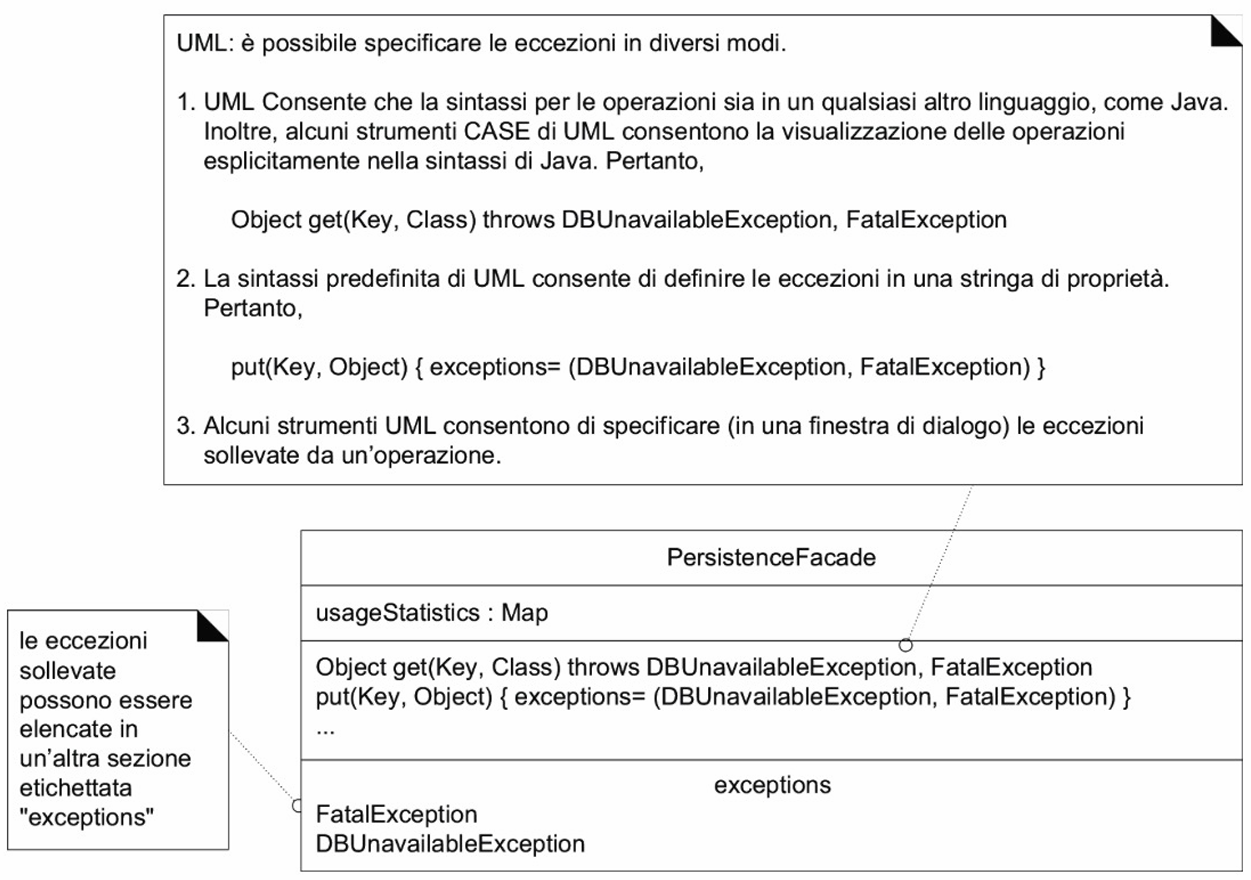
\includegraphics[width=\textwidth]{Esercitazione - Design Patterns/Eccezioni/UML_Eccezioni.png}
            \caption{Eccezioni in un diagramma delle classi}
            \label{fig:immagine1}
        \end{minipage}\hfill
        \begin{minipage}{0.45\textwidth}
            \centering
            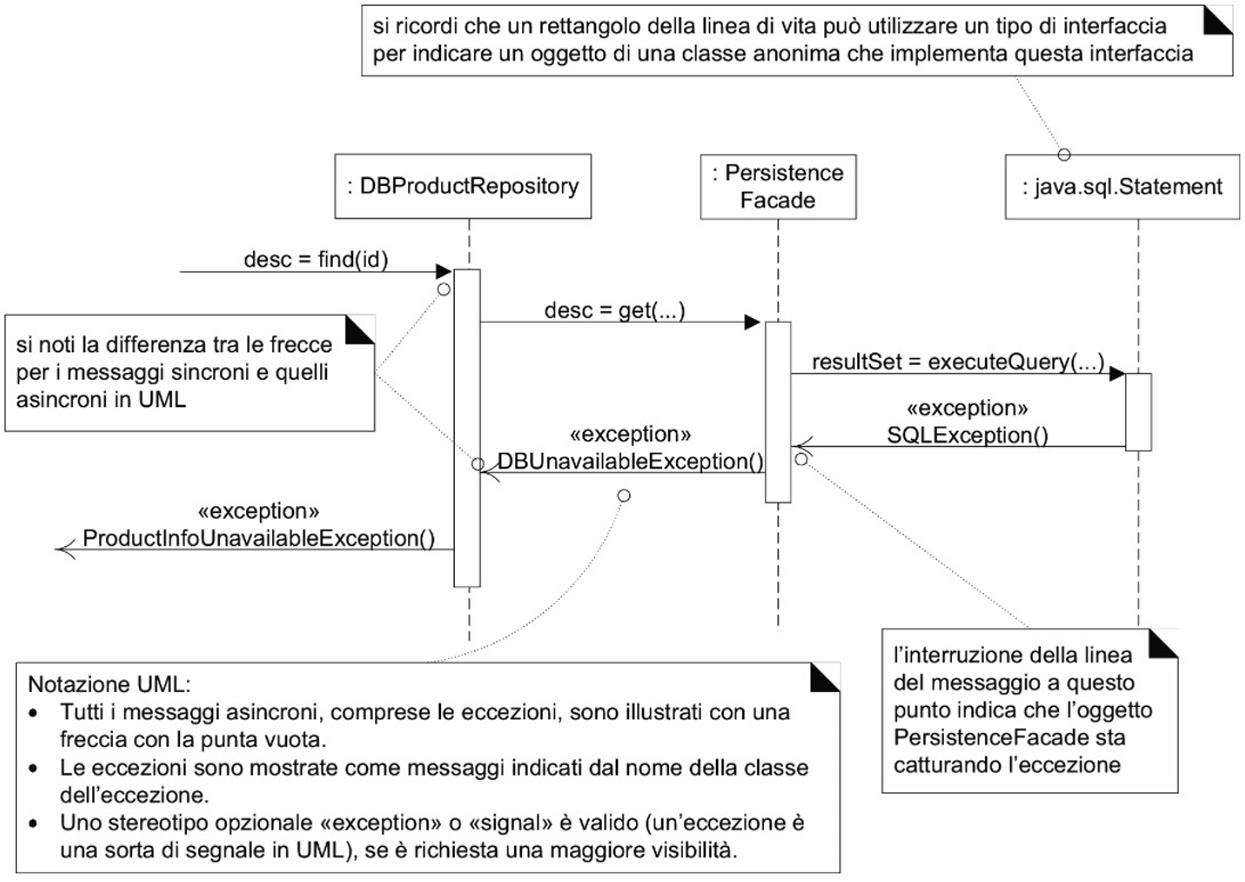
\includegraphics[width=\textwidth]{Esercitazione - Design Patterns/Eccezioni/Diagramma di Sequenza Eccezioni.png}
            \caption{Eccezioni in un diagramma di sequenza}
            \label{fig:immagine2}
        \end{minipage}
    \end{figure}
    \noindent Per gestire l'eccezione, può essere gestita tramite due pattern, il \coloredtext[blue]{\textbf{Centralized Error Logging}} e l'\coloredtext[blue]{\textbf{Error Dialog}}.
    \newpage
    }